\section{Results}

The model performed better than using the average
recipe in predicting the U.S. \gls{UNF}, with
negligible increase in computational time.

\subsection{Depletion Calculation Time and File Size}
For 100 random sets of
burnup and enrichment depletion predictions,
the model takes 0.27 seconds to output discharge composition, while
searching the database for assemblies
with the closest burnup and enrichment (using Pandas)
takes 21.8 seconds. Comparatively, 100 \gls{ORIGEN} calculations
take 118 seconds. Using the model achieves 43,700\% reduction
in time and does not require libraries, or a reactor physics code.
The standalone model pickle file is only
38 Kb, while the curated database (.csv) is 330 Mb.

\subsection{Assembly Comparison}

Ten data points were randomly sampled from the \gls{UDB},
and were compared with the model predictions to observe
two things:
\begin{enumerate}
    \item What isotopes the model is good / bad
        at predicting
    \item What burnup / enrichment range the model is good / bad
        at predicting
\end{enumerate}

Figures \ref{fig:3-2_29998-0}, \ref{fig:3-81_35883-0},
\ref{fig:4-0_35195-0}, and \ref{fig:4-47_50105-0}
show that the model
generally has a high relative error percentage for \textsuperscript{226}Ra
(average concentration $6.0\times10^{-12}\%$),
\textsuperscript{227}Ac (average concentration  $2.3\times10^{-12}\%$), and curium isotopes.
The absolute prediction errors are quite small
(averaging $1e-11$), but the large percent errors are due
to the small value of the data. There was not a notable
difference in the error values for enrichment
and burnup variations.

\begin{figure}
    \centering
    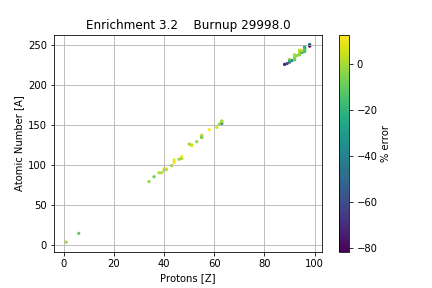
\includegraphics[width=\textwidth]{3-2_29998-0.png}
    \caption{Isotopic composition prediction error for an assembly with 
             $29.998 \frac{GWd}{MT}$ burnup and 3.2  \% enrichment.}
    \label{fig:3-2_29998-0}
\end{figure}

\begin{figure}
    \centering
    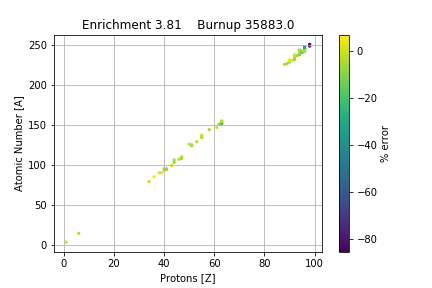
\includegraphics[width=\textwidth]{3-81_35883-0.png}
    \caption{Isotopic composition prediction error for an assembly with 
             $35.883 \frac{GWd}{MT}$ burnup and 3.81  \% enrichment.}
    \label{fig:3-81_35883-0}
\end{figure}

\begin{figure}
    \centering
    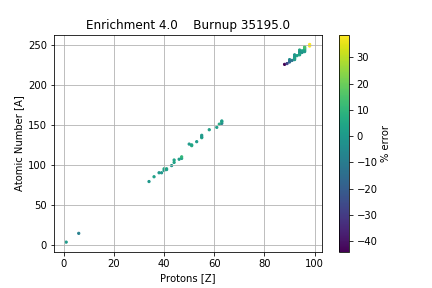
\includegraphics[width=\textwidth]{4-0_35195-0.png}
    \caption{Isotopic composition prediction error for an assembly with 
             $35.193 \frac{GWd}{MT}$ burnup and 4.0 \% enrichment.}
    \label{fig:4-0_35195-0}
\end{figure}


\begin{figure}
    \centering
    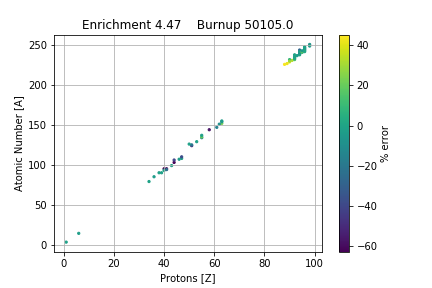
\includegraphics[width=\textwidth]{4-47_50105-0.png}
    \caption{Isotopic composition prediction error for an assembly with 
             $50.105 {GWd}{MT}$ burnup and 4.47  \% enrichment.}
    \label{fig:4-47_50105-0}
\end{figure}

\FloatBarrier

\subsection{U.S. \gls{UNF} Inventory Comparison}

In this section, we compare three \gls{UNF} inventory composition
model approaches.
The only difference is the composition of the
assemblies. The three different inventory compositions were acquired by:

\begin{enumerate}
    \item \textbf{Data}: directly query the assembly composition from the \gls{UDB}.
    \item \textbf{Prediction}: neural network prediction of depleted composition using burnup and enrichment from database
    \item \textbf{Recipe}: using a single composition (recipe) for all assemblies. Assumes all compositions are the same.
\end{enumerate}

The median values for burnup and initial enrichment are
$41,552$ MWd/MT and 3.85 (wt\%), respectively. The concentrations of major
isotopes in the assembly are in Table \ref{tab:avg_assem}.


\begin{table}[h]
    \centering
    \begin{tabular}{|l|r|r|r|r|r|}
        \hline
        Isotopes & $^{235}U$ & $^{238}U$ & $^{239}Pu$ & $^{137}Cs$ & $^{90}Sr$ \\
        \hline
        Concentration [wt\%] & 1.076 & 92.66 & 0.77 & 0.14 & 0.061 \\
        \hline
    \end{tabular}
    \caption{Isotopic concentration of the assembly with median burnup and
             enrichment. This composition is used for the recipe method. 
    \label{tab:avg_assem}}
\end{table}


We compare the three composition predictions according to:
\begin{enumerate}
    \item Isotopic inventory
    \item Waste metrics (activity and decay heat)
    \item Equivalent fissile inventory (equivalent $^{239}Pu$)
\end{enumerate}

The \gls{UDB} contains discharged assembly data
from nuclear reactors in the United States up to May of
2013. We added all the \gls{UNF} assemblies in the database
and evaluated the inventory as it was in 2013. 
Table \ref{tab:met} shows the comparison of the inventories.

\begin{table}[h]
    \centering
    \begin{tabular}{l|r|rr}
        \hline
        Metric & Data & Recipe & Prediction \\
        \hline
        $^{239}Pu$ mass [t] & 320.37 & 351.70 & 321.38\\
        $^{137}Cs$ mass [t] & 63.84 & 66.64 & 63.73 \\
        $^{235}U$ mass [t] & 464.60 & 487.94 & 474.14\\
        $^{238}U$ mass [t] & 42,171 & 42,016 & 42,162\\
        \hline
        Decay Heat [MW] & 193.39 & 198.55 & 193.33 \\
        Activity [$E+21$Bq] & $2.79$ & $2.84$ & $2.75$ \\
        \hline
    \end{tabular}
    \caption{Comparison of \gls{PWR} \gls{UNF} inventory in the U.S,
             obtained from direct data query, recipe approach,
             and neural network prediction. 
    \label{tab:met}}
\end{table}

\FloatBarrier

\subsubsection{Isotopic Inventory}

In terms of isotopic composition accuracy, the trained
neural network model outperforms the
mean recipe method for all isotopes.
Figure \ref{fig:iso_rel} shows the relative
error between the full database, model prediction, and
the mean recipe for
major isotopes. For plutonium isotopes, the trained neural
network model far
outperforms the mean database.

\begin{figure}
    \centering
    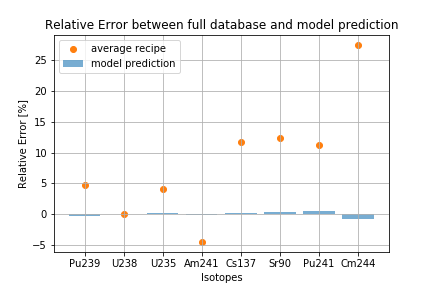
\includegraphics[width=\textwidth]{iso_rel.png}
    \caption{Neural network model prediction error relative to median
             \gls{UDB} recipe, for key isotopes.}
    \label{fig:iso_rel}
\end{figure}


\begin{figure}
    \centering
    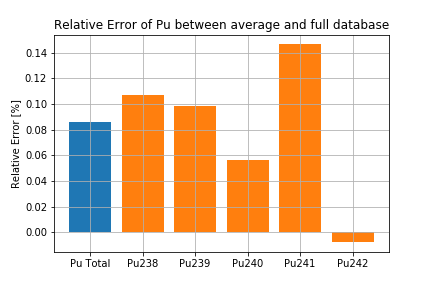
\includegraphics[width=\textwidth]{pu_rel.png}
    \caption{Neural network model prediction error relative to median
             \gls{UDB} recipe, for plutonium isotopes.}
    \label{fig:pu_rel}
\end{figure}

\FloatBarrier


\subsubsection{Waste Management Metrics}
The trained neural network excellently predicts the activity
and decay heat metrics. Figures \ref{fig:assem_dh} and \ref{fig:assem_act}
show the relative error percent of the decay heat and activity
predictions per assembly. The model predicts 99.5\% of
assemblies with an error of less than 1\%.
Figures \ref{fig:assem_dh_recipe} and
\ref{fig:assem_act_recipe} show the relative error
of the decay heat and activity calculated with the average
recipe method.
Unsurprisingly, the error increases as the actual burnup and enrichments
diverge from the average.

\begin{figure}
    \centering
    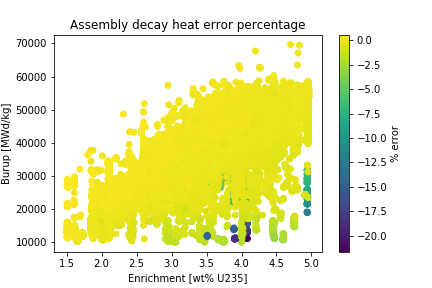
\includegraphics[width=\textwidth]{assem_dh.png}
    \caption{Relative error percentage for predicting the decay
             heat of individual assemblies.}
    \label{fig:assem_dh}
\end{figure}


\begin{figure}
    \centering
    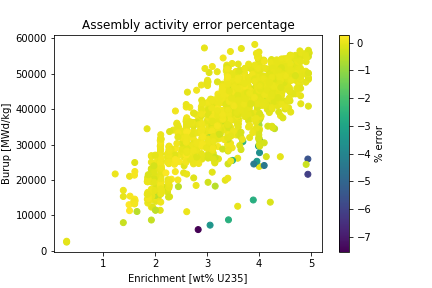
\includegraphics[width=\textwidth]{assem_act.png}
    \caption{Relative error percentage for predicting the
             activity of individual assemblies.}
    \label{fig:assem_act}
\end{figure}



\begin{figure}
    \centering
    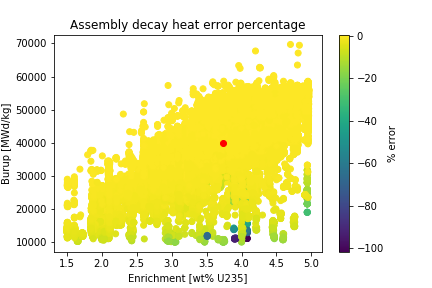
\includegraphics[width=\textwidth]{assem_dh_recipe.png}
    \caption{Relative error in decay heat calculated by the average recipe
             method. The red point is the median enrichment and
             burnup.}
    \label{fig:assem_dh_recipe}
\end{figure}

\begin{figure}
    \centering
    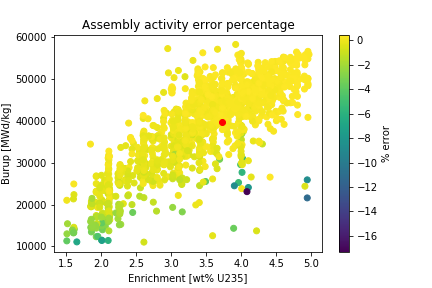
\includegraphics[width=\textwidth]{assem_act_recipe.png}
    \caption{Relative error in activity
             calculated by the average recipe method.
             The red point is the median enrichment and
             burnup.}
    \label{fig:assem_act_recipe}
\end{figure}

\FloatBarrier


Table \ref{tab:wm} shows the decay heat and activity
comparison in the years 2020, 2100, and 3100. The total
error is less than 1.1\% for all metrics at all time periods.
Figure \ref{fig:ha_err} shows relative error in activity and
decay heat as a function of time. It shows
that the model outperforms the average recipe method
in predicting waste metrics.

%! Do the decimal centering
\begin{table}[h]
    \centering
    \begin{tabular}{lcrrr}
        \hline
        Metric & Year & UDB [MW] & Prediction [MW]  & Error [\%] \\
        \hline
        \multirow{3}{*}{\shortstack{Decay \\ Heat }} & 2020 & 40.97 & 41.07 & -0.24 \\
                                                    & 2100 & 16.42 & 16.47 & -0.35 \\
                                                    & 3100 & 3.13 & 3.14 & -0.15 \\
        \hline
         & & UDB [$10^{19}$Bq] & Prediction [$10^{19}$Bq] & Error[\%] \\
        \multirow{3}{*}{\shortstack{Activity}} & 2020 & 46.70 & 46.60 & 0.21 \\
                                               & 2100 & 6.39& 6.38 & 0.07 \\
                                               & 3100 & 0.36 & 0.36 & -0.17 \\
        \hline
    \end{tabular}
    \caption{Decay heat and radioactivity values and errors for years 2020, 2100, and 3100.}
    \label{tab:wm}
\end{table}

\begin{figure}
    \centering
    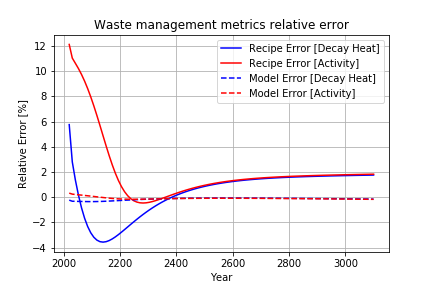
\includegraphics[width=\textwidth]{ha_err.png}
    \caption{Relative error of waste management metrics for \gls{UNF} inventory
             generated by the average recipe and the prediction model.}
    \label{fig:ha_err}
\end{figure}

\FloatBarrier

\subsubsection{Assembly fissile quality}

Fissile quality is frequently quantified in units of 
$^{239}Pu$ equivalent, shown in figure \ref{tab:pu_equiv} \cite{anon_plutonium_1989}. This value is
calculated by aggregating the weighted fissile
values of each isotope in a material. The $^{239}Pu$
equivalent factors are different for fast neutron spectrum 
and thermal neutron spectrum reactors \cite{baker_comparison_1963}
(factors shown in table \ref{tab:pu_equiv}).  
The equivalent fissile value is calculated by:
\begin{gather}
\text{Pu}_{\text{eq}} = \sum_i w_i m_i
\end{gather}
\begin{gather*}
i \in [^{235}U, ^{238}Pu, ^{239}Pu, ^{240}Pu, ^{241}Pu, ^{242}Pu, ^{242}Am] \\
w_i = \text{equivalent weighting factors} \\
m_i = \text{mass of iso i} \\
\end{gather*}
Where the variables represent the mass of each isotope.



\begin{table}[h]
    \centering
    \begin{tabular}{ccc}
        \hline
        & \multirow{2}{*}{\shortstack{LWR \\ (Thermal)}} &
        \multirow{2}{*}{\shortstack{\gls{FBR}\\ (Fast)}} \\ \\
        \hline
        $^{235}U$ & +0.8& +0.8\\
        $^{238}Pu$ & -1.0& +0.44\\
        $^{239}Pu$ & +1.0& +1.0\\
        $^{240}Pu$ & -0.4& +0.14\\
        $^{241}Pu$ & +1.3& +1.5 \\
        $^{242}Pu$ & -1.4& +0.037\\
        $^{241}Am$ & -2.2& -0.33\\
        \hline
    \end{tabular}
    \caption{$^{239}Pu$ equivalence factors from \cite{anon_plutonium_1989}.
             Factors are separately reported for thermal and fast spectra.}
    \label{tab:pu_equiv}
\end{table}


Figure \ref{fig:fiss} shows the fast spectrum $^{239}Pu$ equivalent
value of the \gls{UNF} inventory plotted over time.
The trained model outperforms the recipe method. The
initial falls for all three lines are due to the
decay of plutonium 241, which has a half-life of
14 years.


\begin{figure}
    \centering
    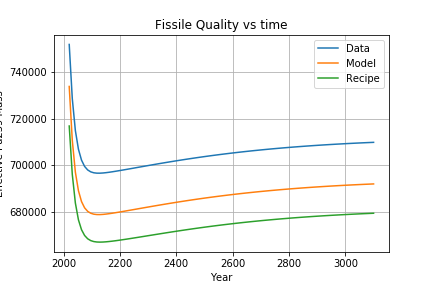
\includegraphics[width=\textwidth]{fiss.png}
    \caption{$^{239}Pu$ equivalent value in time for three
             inventories. The model predictions match closely
             with the value from the database.}
    \label{fig:fiss}
\end{figure}




\subsection{\Cyclus implementation}

In this work, we trained a neural
network model and implemented it as a  \Cyclus reactor
agent that predicts \gls{UNF} composition. The model predicts spent
fuel composition
based on customizable reactor parameters such as
discharge burnup, initial enrichment, cycle time, and power
capacity. The created archetype in \Cyclus also allows users to define
time-dependent
equations instead of constants for reactor parameters.
The user can define an enrichment-burnup matrix for
each assembly in each batch, and the burnup and enrichment
values can be equations in time. This way, users can
implement reactor facilities in which the reactor parameters
change in time (e.g. to represent reactor uprates, industry
burnup trends, etc.).

Figures \ref{fig:cyclus_pu}
and \ref{fig:cyclus_fp} show the discharge fuel composition
of a reactor facility in which we increased the discharge burnup
from 33,000 to 71,710 MWd/MT over 25 discharge cycles.
It should be noted that the model does not take into account
the plausibility of such fuel depletion. For example, it
would be nearly impossible for a  \gls{PWR} to burn 2\%
enriched \gls{UOX} fuel to 70,000 MWd/MT.

The user can also define time-varying
cycle time and refueling time for the reactor model, as shown
in figure \ref{fig:cyclus_time}.


%! it is plutonium in the fuel total
\begin{figure}
    \centering
    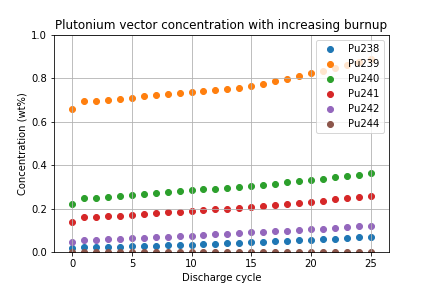
\includegraphics[width=\textwidth]{./cyclus_imp/pu.png}
    \caption{Plutonium isotope composition in discharge fuel over discharge cycle. The model does not predict well for the target burnup values
    that are over the burnup listed in the training dataset.}
    \label{fig:cyclus_pu}
\end{figure}


\begin{figure}
    \centering
    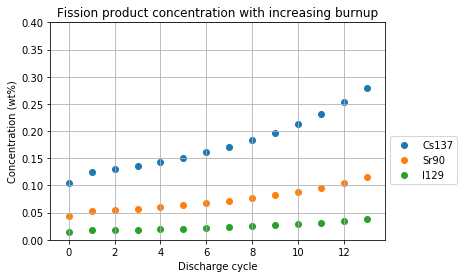
\includegraphics[width=\textwidth]{./cyclus_imp/fp.png}
    \caption{Fission product concentration in discharge fuel over discharge cycle. Increased discharge burnup leads to higher fission product concentration.}
    \label{fig:cyclus_fp}
\end{figure}


\begin{figure}
    \centering
    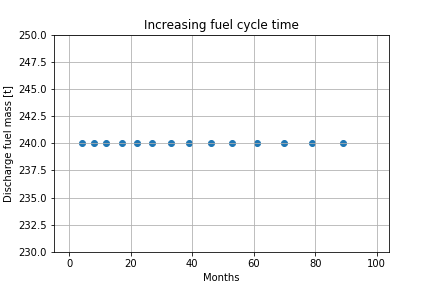
\includegraphics[width=\textwidth]{./cyclus_imp/cycle_time.png}
    \caption{Discharge and refueling cycles can be defined as an equation of time in this reactor archetype. Discharge burnup is scaled to take into account longer fuel residence time, and leads to increase in discharge fuel \textsuperscript{244}Cm composition.
    }
    \label{fig:cyclus_time}
\end{figure}

\subsubsection{Applications and Use Cases}

The capability to set dynamic reactor parameters
allows simulation of various future transition scenarios
that depend on \gls{UNF} inventory characteristics,
such as \gls{MA} inventory. 
Users can simulate future scenarios in which the discharge
burnup of reactors increases over time to reveal
impacts on \gls{MA} inventory and, correspondingly,
transition speed. 

With
advances in materials, reactors may have longer
cycle times and higher fuel discharge burnups.
This dynamic reactor model will be able to account
for the changes in these reactor parameters.
Also, users can simulate potential
power uprates in currently existing fleets, and
estimate corresponding impacts on \gls{UNF} inventory.
\FloatBarrier